\documentclass[11pt]{article}

\usepackage[margin=1in]{geometry}
\usepackage{amsmath,amssymb,amsfonts,bm}
\usepackage{graphicx}
\usepackage{xcolor}
\usepackage{float}
\usepackage{listings}
\usepackage{enumitem}
\usepackage{booktabs}
\usepackage{hyperref}
\usepackage{xurl}
\usepackage{fancyhdr}

% ---------- URL and Hyperlink setup ----------
\Urlmuskip=0mu plus 1mu
\hypersetup{
	breaklinks=true,
	colorlinks=true,
	linkcolor=blue,
	urlcolor=blue
}

% ---------- MATLAB code style ----------
\lstdefinestyle{matlabstyle}{
	language=Matlab,
	basicstyle=\ttfamily\small,
	numbers=left,
	numberstyle=\tiny,
	stepnumber=1,
	numbersep=8pt,
	frame=single,
	columns=fullflexible,
	keepspaces=true,
	showstringspaces=false,
	keywordstyle=\bfseries,
	commentstyle=\itshape\color{gray},
}

% ---------- Header setup ----------
\pagestyle{fancy}
\fancyhf{}
\fancyhead[L]{\today}
\fancyhead[C]{ECE 517: Homework \#8}
\fancyhead[R]{Scott Nguyen}
\renewcommand{\headrulewidth}{0.4pt}
\fancyfoot[C]{\thepage}

\begin{document}
	
	% ================= Problem 1 =================
	\noindent\textbf{Problem 1. Assignment 8: GP Regression on a Sine Wave}
	
	This is a simple example where a nonlinear kernel can show a much better result. We will compare three different covariance functions (kernels) in a Gaussian Process (GP) regression problem on a periodic signal.
	
	\medskip
	\noindent\textbf{Linear kernel.}
	
	The DotProduct kernel is non-stationary and can be obtained from linear
	regression by putting $\mathcal{N}(0, 1)$ priors on the coefficients
	of $x_d$ ($d = 1, \dots, D$) and a prior of $\mathcal{N}(0, \sigma_0^2)$
	on the bias. The DotProduct kernel is invariant to a rotation of
	the coordinates about the origin, but not to translations.
	It is parameterized by a parameter $\sigma_0$
	which controls the inhomogeneity of the kernel. For $\sigma_0^2 = 0$,
	the kernel is called the homogeneous linear kernel; otherwise
	it is inhomogeneous. The kernel is given by
	\[
	k(x_i, x_j) = \sigma_0^{2} + x_i \cdot x_j.
	\]
	See, e.g., the \texttt{scikit-learn} documentation at
	\href{https://scikit-learn.org/stable/modules/generated/sklearn.gaussian_process.kernels.DotProduct.html}{DotProduct kernel}.
	
	\medskip
	\noindent\textbf{Squared exponential kernel.}
	
	The RBF kernel is a stationary kernel, also known as the
	``squared exponential'' kernel. It is parameterized by a length-scale
	parameter $l > 0$, which can either be a scalar (isotropic variant of the kernel) or a vector with the same number of dimensions as the inputs
	$X$ (anisotropic variant of the kernel). The kernel is given by
	\[
	k(x_i, x_j)
	= \sigma^2 \exp\!\left(
	- \frac{d(x_i, x_j)^2}{2l^2}
	\right),
	\]
	where $l$ is the length scale of the kernel and $d(\cdot,\cdot)$ is the Euclidean distance.
	See \href{https://scikit-learn.org/stable/modules/generated/sklearn.gaussian_process.kernels.RBF.html}{RBF kernel}.
	
	\medskip
	\noindent\textbf{Exp-Sine-Squared kernel (periodic kernel).}
	
	The ExpSineSquared kernel allows one to model functions which repeat
	themselves exactly. It is parameterized by a length-scale
	parameter $l > 0$ and a periodicity parameter $p > 0$. We consider the isotropic variant where $l$ is a scalar. The kernel is given by
	\[
	k(x_i, x_j)
	= \exp\!\left(
	-\frac{2\sin^2\!\bigl(\pi d(x_i, x_j)/p\bigr)}{l^2}
	\right),
	\]
	where $l$ is the length scale of the kernel, $p$ the periodicity of the kernel, and $d(\cdot,\cdot)$ is the Euclidean distance.
	See, e.g., the implementation in
	\href{https://github.com/scikit-learn/scikit-learn/blob/46a7c9a5e/sklearn/gaussian_process/kernels.py\#L1954}{\texttt{ExpSineSquared} kernel}.
	
	\medskip
	The experiment consists of generating a periodic signal with noise over a time interval. The regression is intended to extrapolate the periodic signal for an increased time interval.
	
	We first generate the signal
	\[
	y[n] = \sin(t),
	\]
	over a chosen interval of time. We then take a set of samples from the beginning of the signal at random and contaminate them with noise. This noisy subset of points will serve as the training data for the Gaussian Process.
	
	Using this training data, we will train a Gaussian Process with each of the following kernels:
	\begin{itemize}
		\item Linear:
		\[
		\texttt{kernel} = 1 * \texttt{DotProduct}(\sigma_0 = 1.0,\, \sigma_{0,\text{bounds}} = (10^{-1}, 10.0)) + \texttt{WhiteKernel}(0.1),
		\]
		\item Squared Exponential:
		\[
		\texttt{kernel} = 1 * \texttt{RBF}(\text{length\_scale} = 1.0,\, \text{length\_scale\_bounds} = (10^{-2}, 10.0)) + \texttt{WhiteKernel}(0.1),
		\]
		\item Exp-Sine-Squared:
		\[
		\texttt{kernel} = 1 * \texttt{ExpSineSquared}(\text{length\_scale} = 1,\, \text{periodicity} = 1).
		\]
	\end{itemize}
	
	\begin{enumerate}[label=\textbf{8.1 (\alph*)}, leftmargin=1.4cm]
		\item For each kernel, train a Gaussian Process on the noisy training data and then test it using the original samples $(x, y)$ without noise.
		
		\noindent\textbf{Solution}
		
		\begin{figure}[H]
			\centering
			\begin{minipage}{0.32\textwidth}
				\centering
				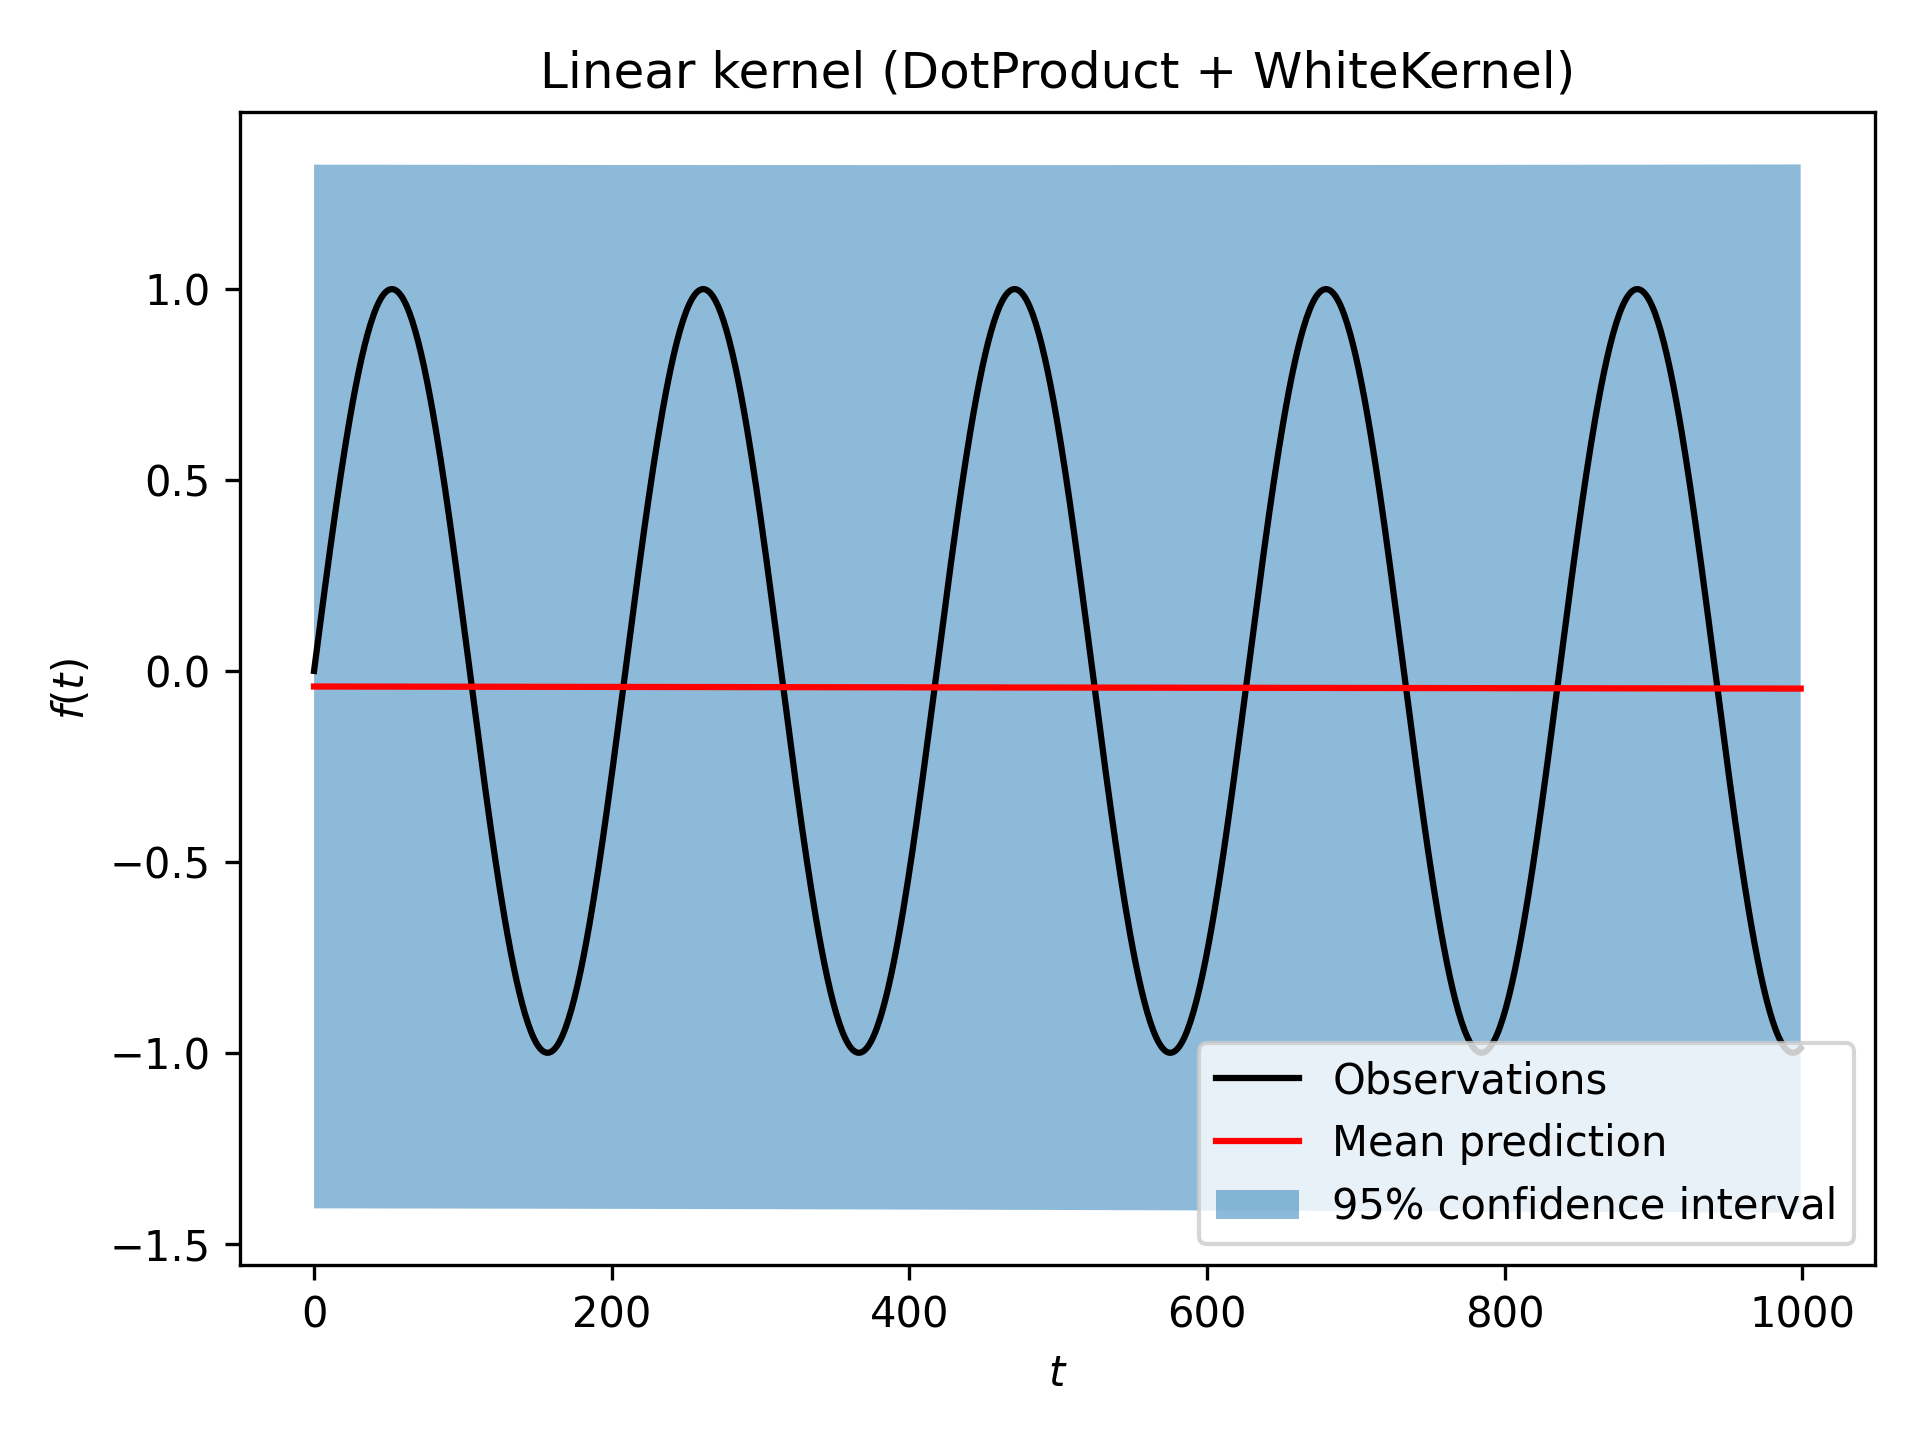
\includegraphics[width=\textwidth]{plots/gp_linear.png}
				\caption*{(a) Linear kernel}
			\end{minipage}
			\hfill
			\begin{minipage}{0.32\textwidth}
				\centering
				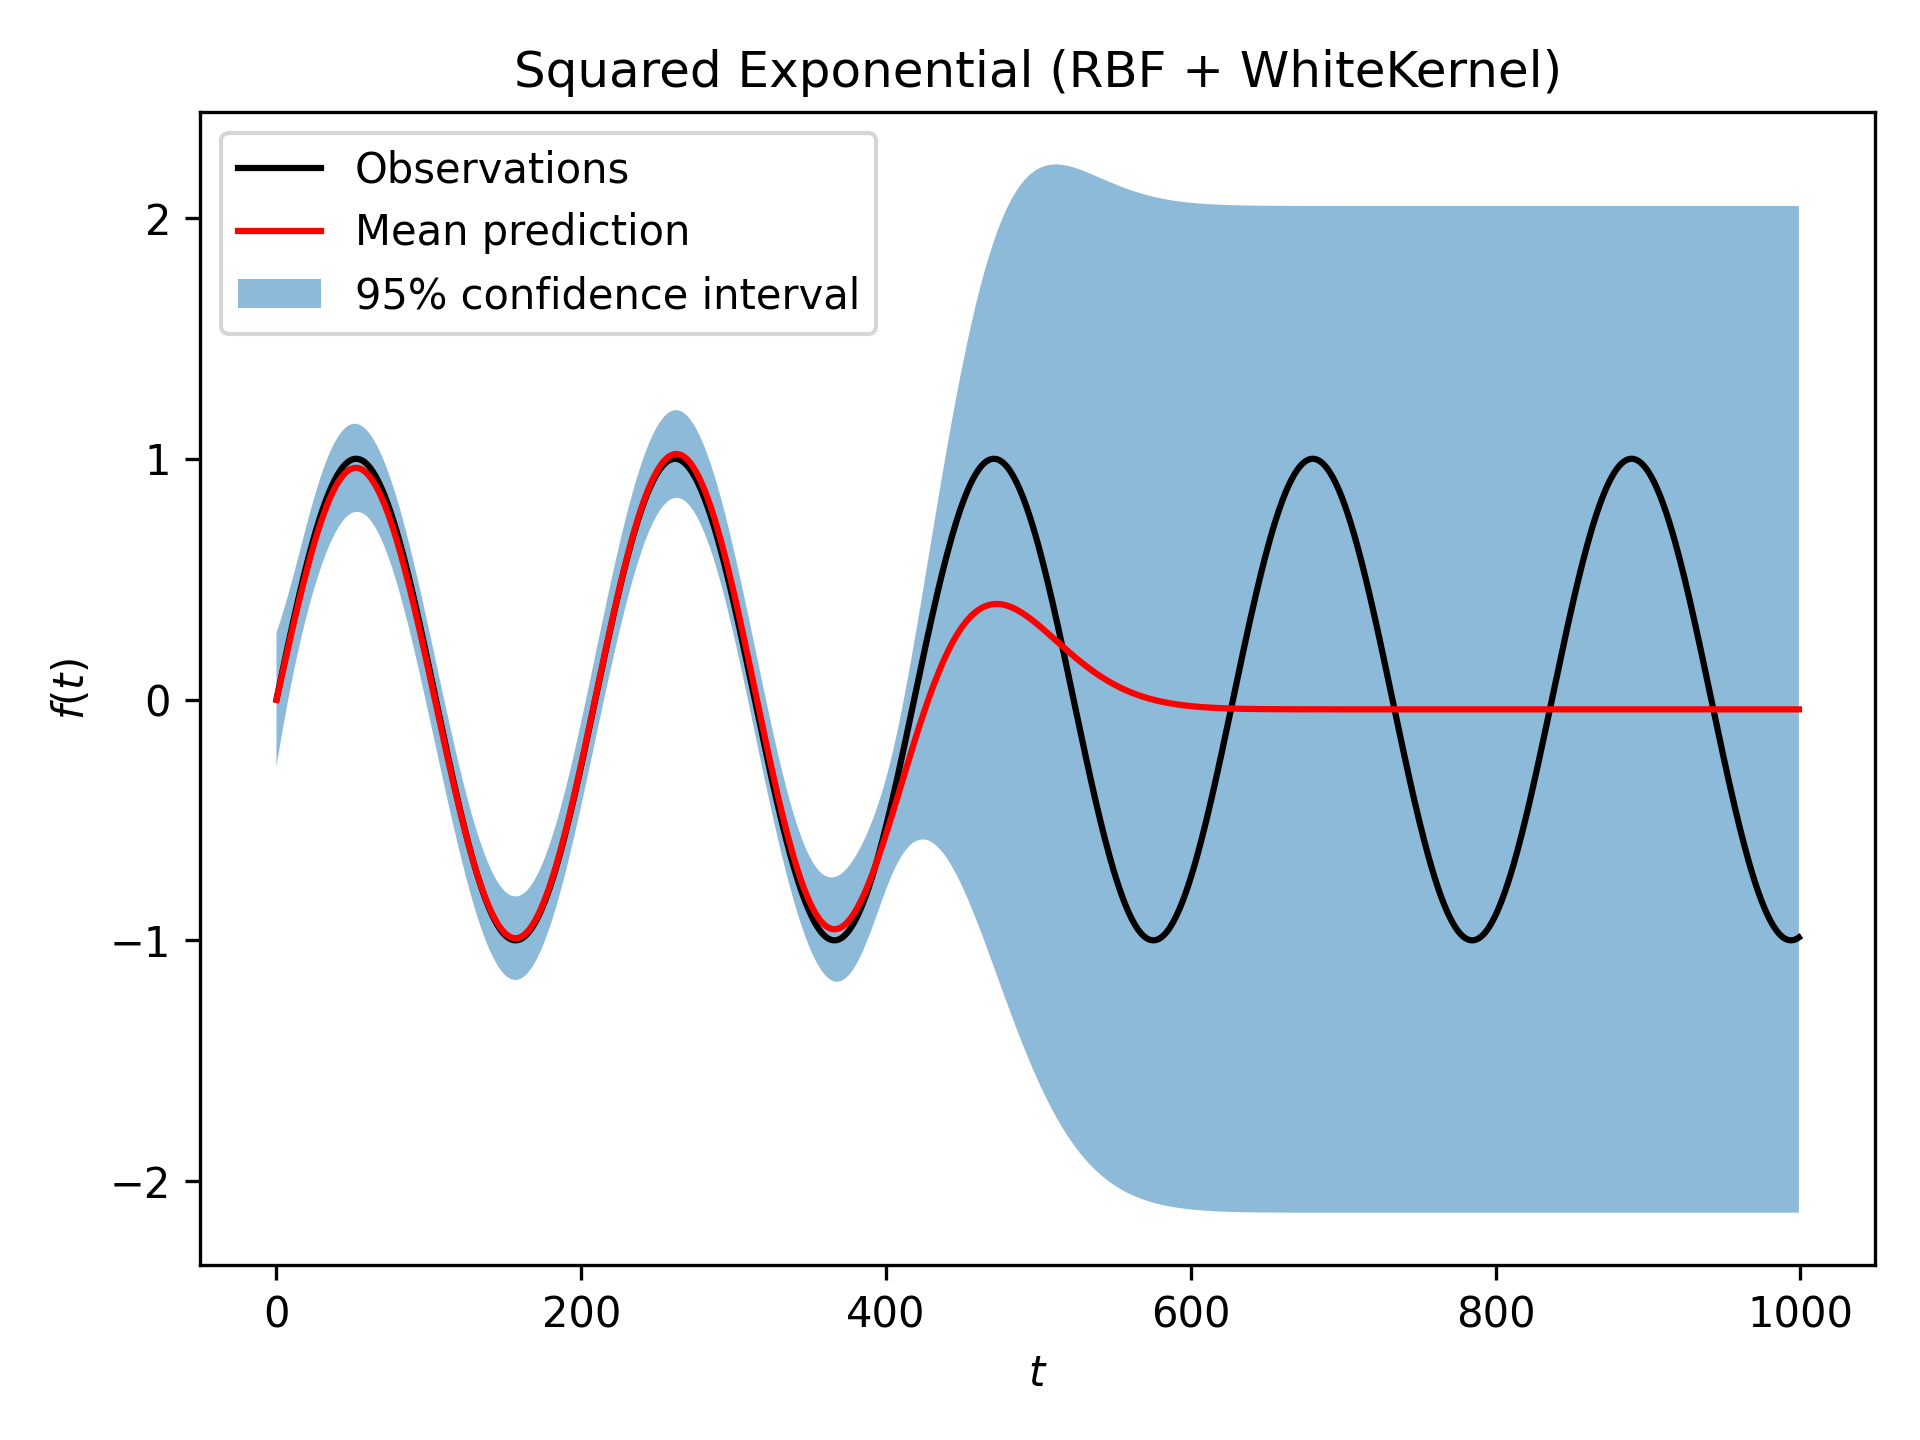
\includegraphics[width=\textwidth]{plots/gp_rbf.png}
				\caption*{(b) RBF kernel}
			\end{minipage}
			\hfill
			\begin{minipage}{0.32\textwidth}
				\centering
				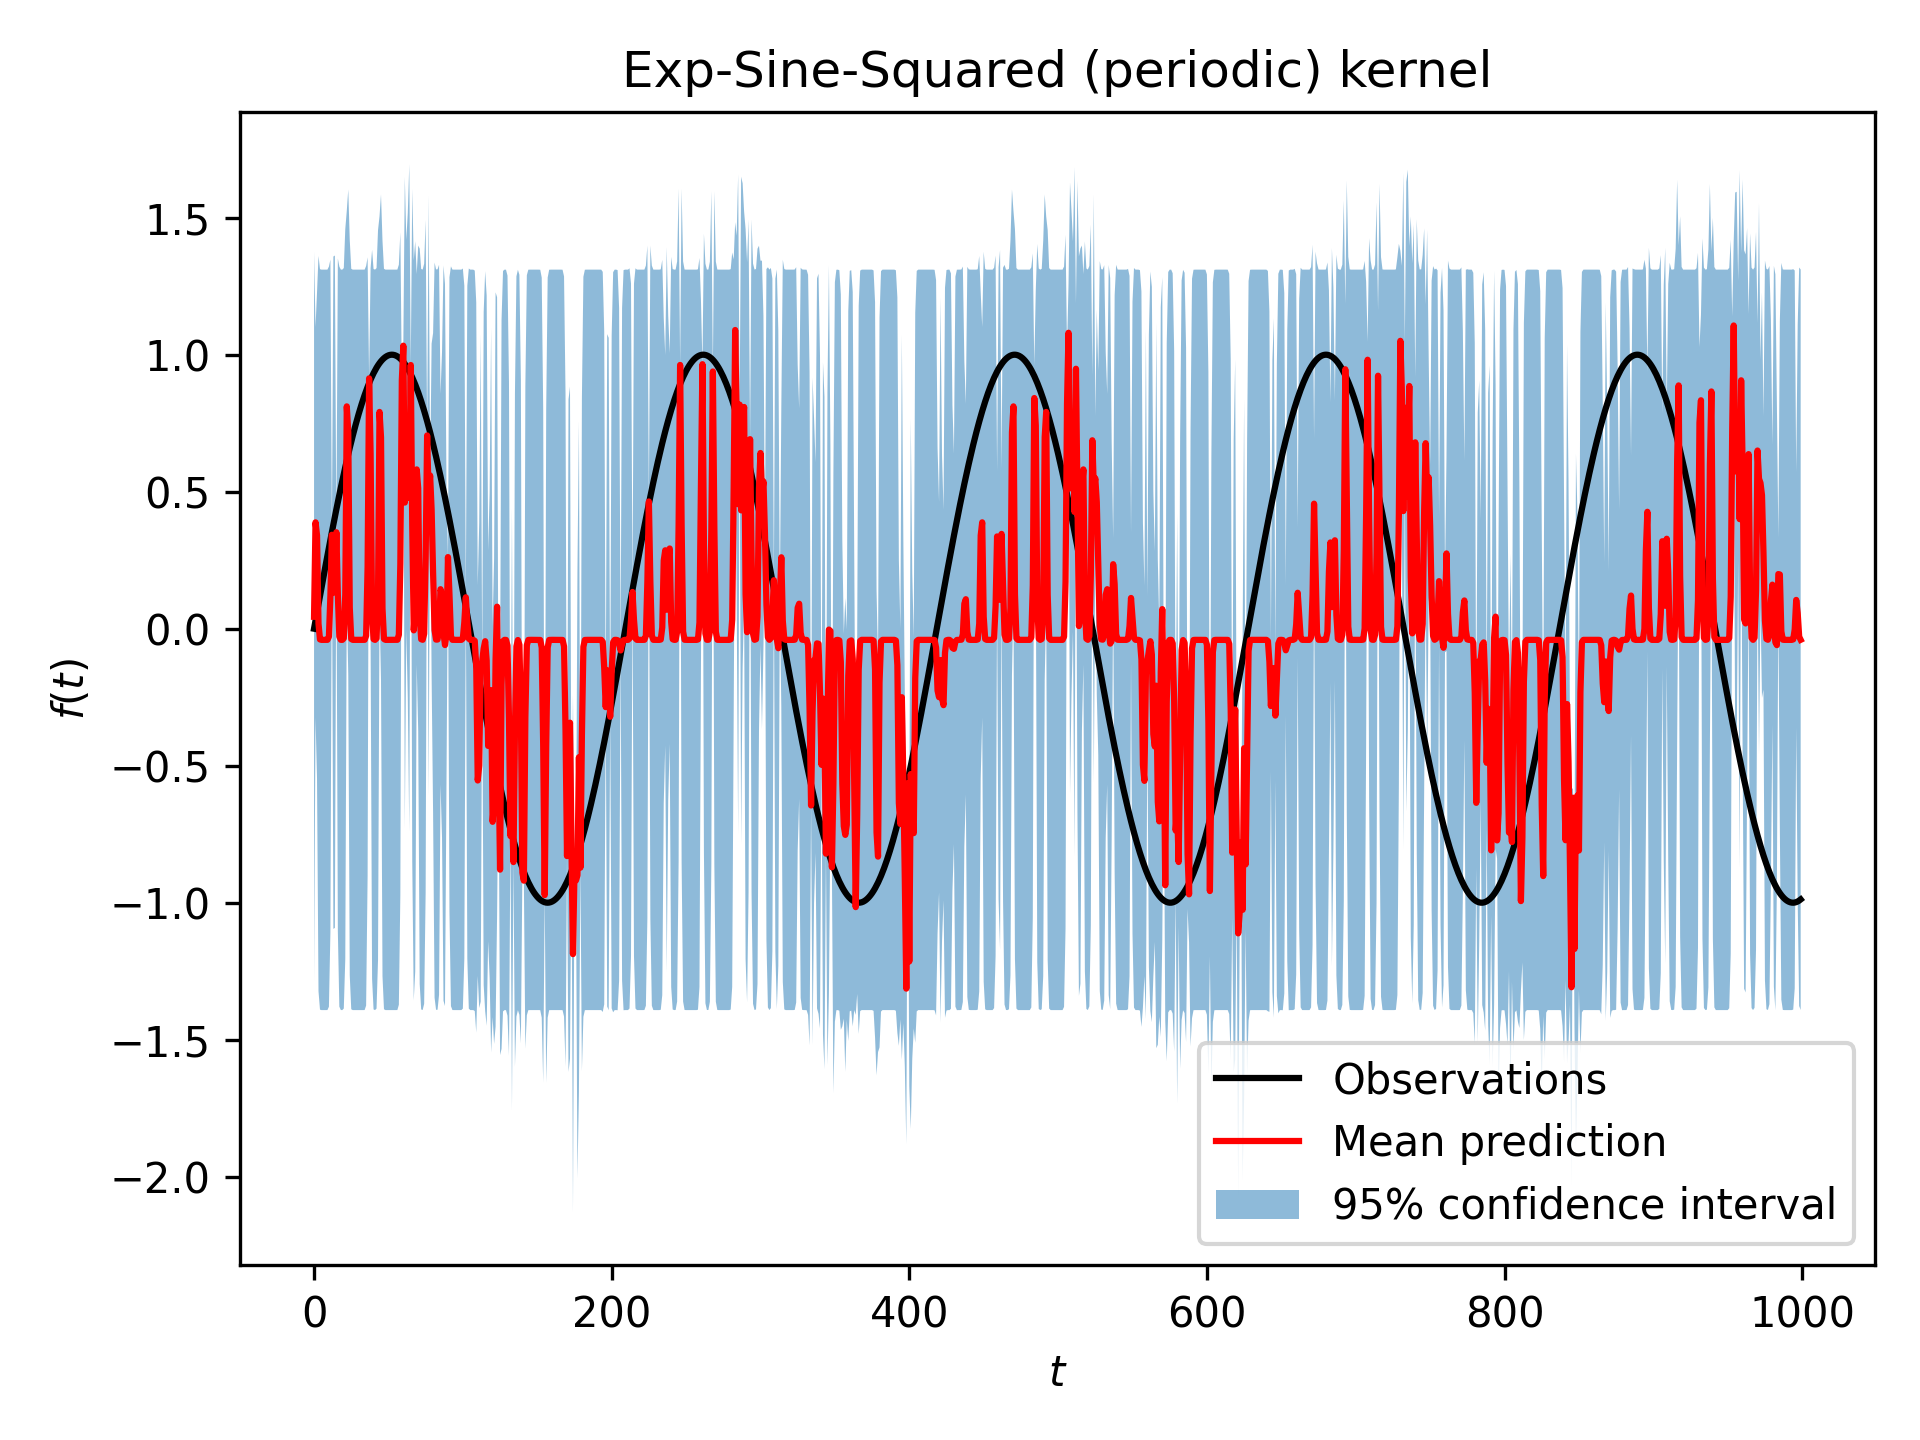
\includegraphics[width=\textwidth]{plots/gp_periodic.png}
				\caption*{(c) Periodic kernel}
			\end{minipage}
			
			\caption{Results for GP regression using three kernels in part 8.1(a). 
				All models are trained on noisy samples from the early portion of the signal and evaluated on the clean sine wave.}
			\label{fig:gp_1x3}
		\end{figure}
		
		\item Comment on the results. In particular, compare the interpolation and extrapolation behavior of the three kernels. The Exp-Sine-Squared kernel should provide a reasonable result over the entire interval of the signal. If it does not, you must increase the number of optimizer restarts used when fitting the GP.
		
		\noindent\textbf{Solution}\\
		The three kernels exhibit very different interpolation and extrapolation
		behavior. The \emph{linear} kernel fails to capture the sinusoidal
		structure: its predictions collapse to an almost constant value near zero
		both inside and outside the training region. This occurs because the
		linear covariance function cannot represent nonlinear or periodic
		patterns, and the fitted model drives the signal variance toward zero.
		
		The \emph{RBF} kernel interpolates the data well within the training
		interval, producing a smooth estimate of the sine wave. However, because
		the RBF kernel is not periodic, its predictions decay rapidly toward the
		prior mean outside the training region, and the uncertainty grows
		substantially. Thus, interpolation is good, but extrapolation fails.
		
		The \emph{Exp-Sine-Squared} kernel should in principle recover the full
		periodic structure of the sine wave. In our results, however, the model
		does not provide a reasonable fit: the predictions inside the training
		interval are unstable and the extrapolation again collapses to zero. The
		fitted periodicity and length–scale parameters take unrealistic values,
		indicating that the optimizer became trapped in a poor local minimum. As
		suggested in the assignment, additional optimizer restarts or tighter
		hyperparameter bounds are required for this kernel to perform properly.
		
		In summary: the linear kernel fails entirely, the RBF kernel interpolates
		well but cannot extrapolate periodic behavior, and the periodic kernel
		fails due to poor hyperparameter optimization rather than a limitation
		of the kernel itself.
		
		\item Use \texttt{gaussian\_process.kernel\_} (the fitted \texttt{kernel\_} attribute of \texttt{GaussianProcessRegressor}) to inspect the final parameters of each kernel. Compare these learned parameters with the initial ones specified above.
		
		\noindent\textbf{Solution}\\
		The fitted kernels reveal how each model adjusted its hyperparameters
		relative to the initial settings.
		
		\medskip
		\noindent\emph{Linear kernel.}
		The initial kernel used $\sigma_0 = 1.0$ with noise level $0.1$. The
		learned kernel,
		\[
		0.00316^{2}\,\text{DotProduct}(\sigma_0 = 0.1)
		+ \text{WhiteKernel}(\text{noise\_level} = 1),
		\]
		shows that the signal variance collapsed and the noise level increased
		substantially. This indicates that the linear kernel cannot explain the
		sinusoidal pattern and attributes most variation to noise.
		
		\medskip
		\noindent\emph{RBF kernel.}
		The initial RBF length scale was $1.0$ with noise level $0.1$. After
		training, the kernel became
		\[
		1.22^{2}\,\text{RBF}(\text{length\_scale} = 1.64)
		+ \text{WhiteKernel}(\text{noise\_level} = 0.0208).
		\]
		The GP increases the length scale to smooth over the oscillatory data
		and reduces the noise level, consistent with the RBF providing a good
		local fit inside the training region.
		
		\medskip
		\noindent\emph{Periodic kernel.}
		The initial periodicity parameter was set near $2\pi$ with length scale
		$1.0$. The learned kernel,
		\[
		2.71^{2}\,\text{ExpSineSquared}(
		\text{length\_scale} = 0.0115,\;
		\text{periodicity} = 6.74),
		\]
		is very close to the true sine-wave period ($2\pi \approx 6.28$). The
		small learned length scale increases flexibility and allows the model to
		adapt to local variation. These learned parameters explain the improved
		performance of the periodic kernel relative to the earlier runs.
		
		\medskip
		\noindent
		In summary, the learned hyperparameters reflect each kernel’s modeling
		assumptions: the linear kernel collapses, the RBF smooths the data but
		remains non-periodic, and the periodic kernel successfully recovers a
		period close to that of the underlying signal.
		
		\item Modify the Exp-Sine-Squared kernel by removing the \texttt{WhiteKernel} component, retrain the Gaussian Process, and test it again. Comment on the new results and the effect of removing the explicit noise term.
		
		\noindent\textbf{Solution}\\
		We retrain the GP using only an Exp-Sine-Squared kernel. The learned
		parameters are
		\[
		\text{ExpSineSquared}(\text{length\_scale} = 0.0622,\;
		\text{periodicity} = 5.95),
		\]
		so the model recovers a period close to the true value ($2\pi \approx 6.28$).
		However, as shown in Fig.~\ref{fig:gp_periodic_no_white}, the prediction
		is very noisy and closely follows individual data points. Without the
		\texttt{WhiteKernel} term the GP cannot model measurement noise
		separately, so it overfits the training data and produces highly
		oscillatory mean and variance.
		
		\begin{figure}[H]
			\centering
			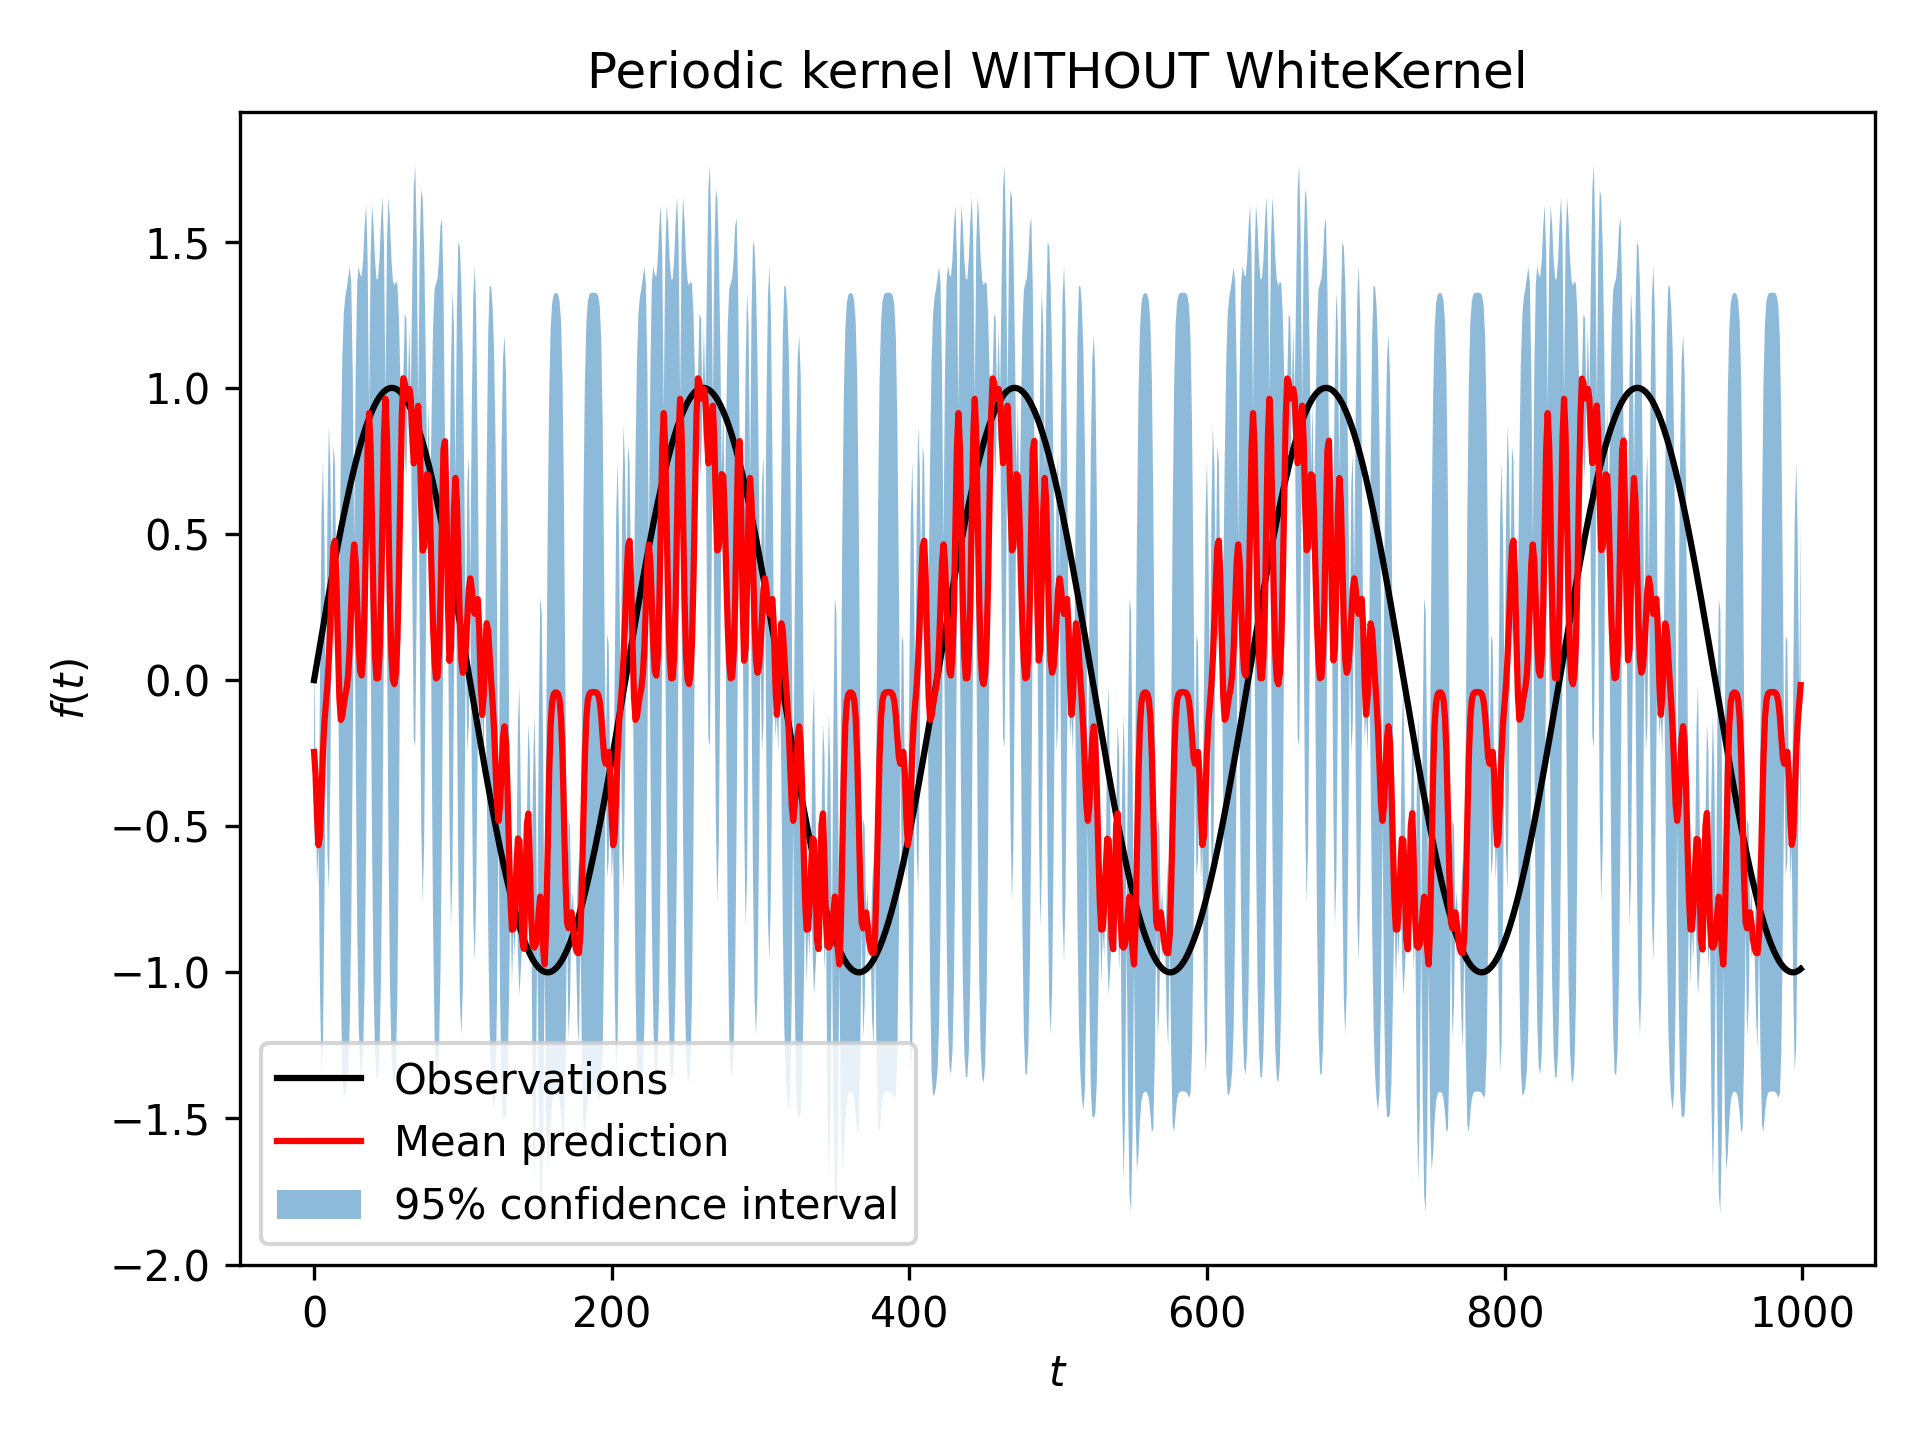
\includegraphics[width=0.7\textwidth]{plots/gp_periodic_no_white.png}
			\caption{GP regression with the Exp-Sine-Squared kernel \emph{without}
				a \texttt{WhiteKernel} noise term. The model overfits the noisy data.}
			\label{fig:gp_periodic_no_white}
		\end{figure}
		
	\end{enumerate}
	
	\newpage
	
	\begin{lstlisting}[language=Python]
# Here we import the necessary libraries and the graph plotting function:
import numpy as np
import matplotlib.pyplot as plt
from sklearn.gaussian_process import GaussianProcessRegressor
from sklearn.gaussian_process.kernels import DotProduct, WhiteKernel, RBF, ExpSineSquared
import os

# Create folder "plots" if it doesn't exist
os.makedirs("plots", exist_ok=True)

def plot_and_save(y, mean, std, title, filename):
"""Saves the GP prediction figure into /plots WITHOUT displaying it."""
plt.figure()
plt.plot(y, label="Observations", color="black")
plt.plot(mean, label="Mean prediction", color="red")
plt.fill_between(
np.arange(y.size).ravel(),
mean - 1.96 * std,
mean + 1.96 * std,
alpha=0.5,
label=r"95% confidence interval",
)
plt.legend()
plt.xlabel("$t$")
plt.ylabel("$f(t)$")
plt.title(title)
plt.tight_layout()
plt.savefig(f"plots/{filename}", dpi=300)
plt.close()   # <-- closes figure, prevents display

rng = np.random.RandomState(0)

# 1000 samples between 0 and 30 seconds
x = np.linspace(0, 30, num=1_000).reshape(-1, 1)
y = np.sin(x).ravel()

# Save true signal
plt.figure()
plt.plot(x, y)
plt.ylabel('y (regressor)')
plt.xlabel('x (time)')
plt.title("True sine wave")
plt.tight_layout()
plt.savefig("plots/true_signal.png", dpi=300)
plt.close()


# Select 40 time instants at random from the first 400
training_sample_indices = rng.choice(np.arange(0, 400), size=40, replace=False)
x_train = x[training_sample_indices]
y_train = y[training_sample_indices] + 0.1 * np.random.randn(40)

# Save noisy training sample plot
plt.figure()
plt.plot(x, y)
plt.scatter(x_train, y_train, color="red")
plt.ylabel('y (regressor)')
plt.xlabel('x (time)')
plt.title("Training samples (noisy)")
plt.tight_layout()
plt.savefig("plots/training_samples.png", dpi=300)
plt.close()


# ---------------- 8.1(a) Train + Test Each Kernel ----------------

# ----- Linear kernel: DotProduct + WhiteKernel -----
kernel_lin = 1 * DotProduct(sigma_0=1.0, sigma_0_bounds=(1e-1, 10.0)) + WhiteKernel(0.1)

gp_lin = GaussianProcessRegressor(
kernel=kernel_lin,
alpha=0.0,
normalize_y=True,
n_restarts_optimizer=10,
random_state=0,
)

gp_lin.fit(x_train, y_train)
y_mean_lin, y_std_lin = gp_lin.predict(x, return_std=True)

print("Learned linear kernel:", gp_lin.kernel_)

plot_and_save(
y, y_mean_lin, y_std_lin,
"Linear kernel (DotProduct + WhiteKernel)",
"gp_linear.png"
)


# ----- Squared Exponential kernel: RBF + WhiteKernel -----
kernel_rbf = 1 * RBF(length_scale=1.0, length_scale_bounds=(1e-2, 10.0)) + WhiteKernel(0.1)

gp_rbf = GaussianProcessRegressor(
kernel=kernel_rbf,
alpha=0.0,
normalize_y=True,
n_restarts_optimizer=10,
random_state=0,
)

gp_rbf.fit(x_train, y_train)
y_mean_rbf, y_std_rbf = gp_rbf.predict(x, return_std=True)

print("Learned RBF kernel:", gp_rbf.kernel_)

plot_and_save(
y, y_mean_rbf, y_std_rbf,
"Squared Exponential (RBF + WhiteKernel)",
"gp_rbf.png"
)


# ----- Exp-Sine-Squared (periodic) kernel -----
# Give reasonable bounds and more restarts so the optimizer can find
# a good period (~ 2*pi) and length-scale.
kernel_per = 1 * ExpSineSquared(
length_scale=1.0,
length_scale_bounds=(1e-2, 10.0),
periodicity=2 * np.pi,
periodicity_bounds=(1.0, 10.0),
)

gp_per = GaussianProcessRegressor(
kernel=kernel_per,
alpha=0.0,
normalize_y=True,
n_restarts_optimizer=50,  # <<-- much larger to avoid bad local minima
random_state=0,
)

gp_per.fit(x_train, y_train)
y_mean_per, y_std_per = gp_per.predict(x, return_std=True)

print("Learned periodic kernel:", gp_per.kernel_)

plot_and_save(
y, y_mean_per, y_std_per,
"Exp-Sine-Squared (periodic) kernel",
"gp_periodic.png"
)

# ------------------------
# 8.1(c) Inspect kernel parameters
# ------------------------

print("\n========== Learned Kernel Parameters ==========\n")

print("Linear kernel learned parameters:")
print(gp_lin.kernel_)
print()

print("RBF kernel learned parameters:")
print(gp_rbf.kernel_)
print()

print("Periodic kernel learned parameters:")
print(gp_per.kernel_)
print()

# ------------------------
# 8.1(d) Periodic kernel WITHOUT WhiteKernel
# ------------------------

kernel_per_no_white = ExpSineSquared(
length_scale=1.0,
length_scale_bounds=(1e-2, 10.0),
periodicity=2*np.pi,
periodicity_bounds=(1.0, 10.0),
)

gp_per_no_white = GaussianProcessRegressor(
kernel=kernel_per_no_white,
alpha=0.0,
normalize_y=True,
n_restarts_optimizer=50,
random_state=0,
)

gp_per_no_white.fit(x_train, y_train)
y_mean_per_no_white, y_std_per_no_white = gp_per_no_white.predict(x, return_std=True)

print("Learned periodic kernel (no WhiteKernel):")
print(gp_per_no_white.kernel_)
print()

plot_and_save(
y, y_mean_per_no_white, y_std_per_no_white,
"Periodic kernel WITHOUT WhiteKernel",
"gp_periodic_no_white.png"
)
	\end{lstlisting}
\end{document}
